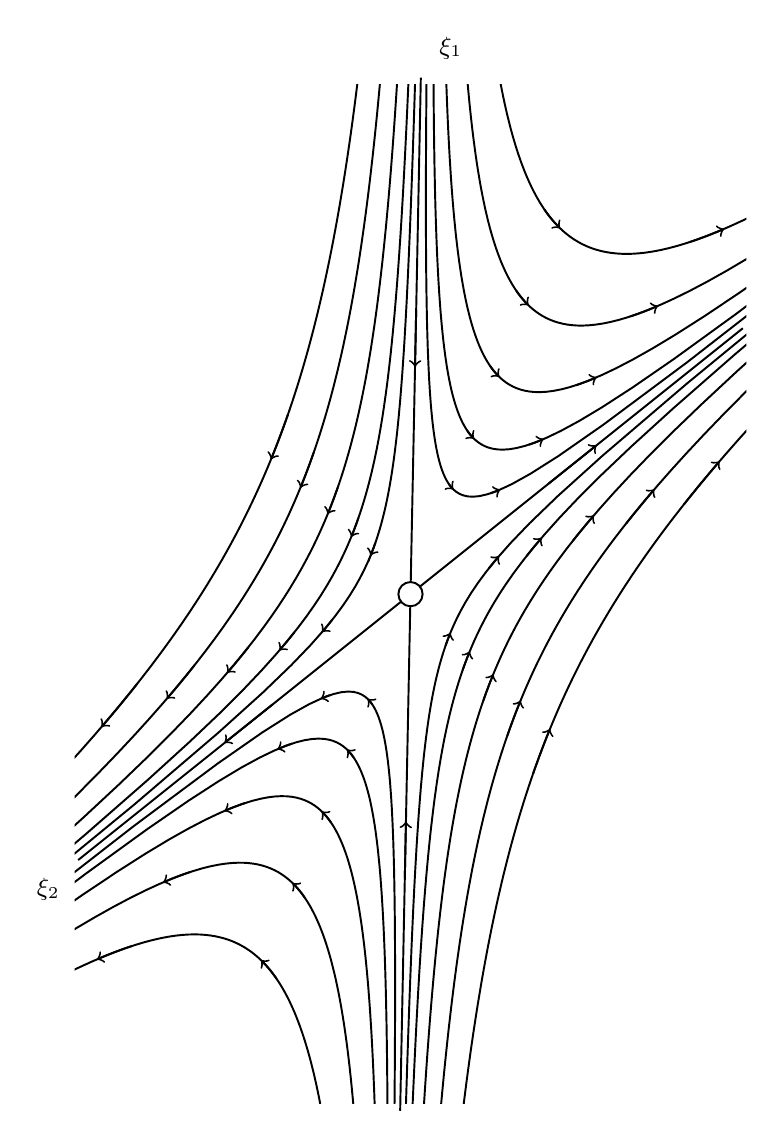
\begin{tikzpicture}[scale=2.5729,font=\small,x=0.85cm,y=0.85cm,line width=0.7pt]
  % Saddle: u'=-u, v'=v; h_1=(0.02,1), h_2=(-1,-0.8).
  % Thus x=0.02u-v, y=u-0.8v and u*v is constant along each orbit.
  \begin{scope}
    \clip (-1.95,-2.96) rectangle (1.95,2.96);
    \foreach \su in {-1,1} {
      \foreach \sv in {-1,1} {
        \foreach \k in {0.10,0.22,0.43,0.76,1.22} {
          \draw plot[domain=0.035:6,samples=220,variable=\s]
            ({0.02*\su*\s-\sv*\k/\s},
             {\su*\s-0.8*\sv*\k/\s});
          \foreach \m in {0.65,1.40} {
            \draw[->] plot[domain={1.06*\m*sqrt(\k)}:{0.94*\m*sqrt(\k)},
              samples=9,variable=\s]
              ({0.02*\su*\s-\sv*\k/\s},
               {\su*\s-0.8*\sv*\k/\s});
          }
        }
      }
    }
  \end{scope}
  \draw (-0.060,-3)--(0.060,3);
  \draw (-1.93,-1.544)--(1.93,1.544);
  \foreach \sgn in {-1,1} {
    \draw[->] ({0.02*1.65*\sgn},{1.65*\sgn})
      --({0.02*1.32*\sgn},{1.32*\sgn});
    \draw[->] ({0.80*\sgn},{0.64*\sgn})
      --({1.08*\sgn},{0.864*\sgn});
  }
  \fill[white] (0,0) circle (1.7pt);
  \draw (0,0) circle (1.7pt);
  \node[above right=3pt] at (0.060,3) {$\xi_1$};
  \node[below left=3pt] at (-1.93,-1.544) {$\xi_2$};
\end{tikzpicture}
